\begin{figure}[t]
    \centering
    \begin{subfigure}[t]{\linewidth}
    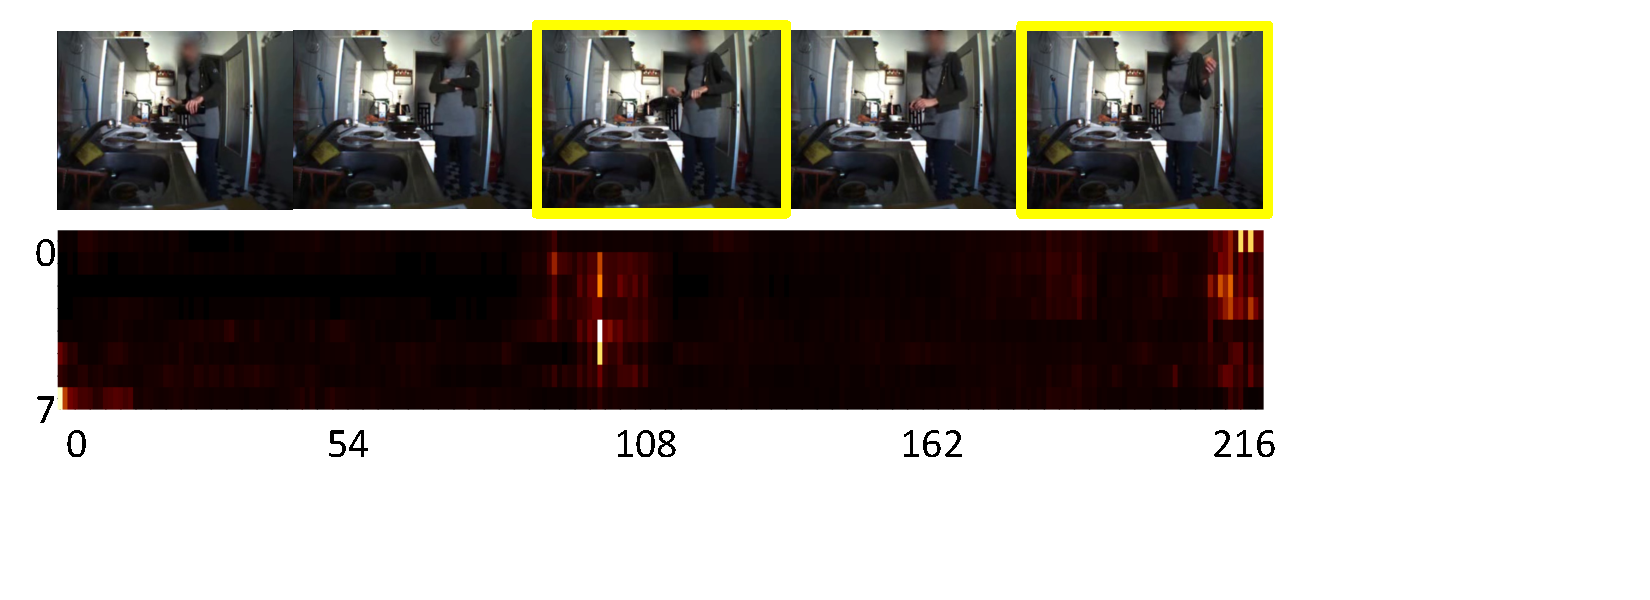
\includegraphics[width=\columnwidth]{Figures/pdf/attn_vis_fe2.pdf}
    \caption{Activity: Fried egg}
    \label{fig:4a}
    \end{subfigure}
    \begin{subfigure}[t]{\linewidth}
    % \vspace{1mm}
    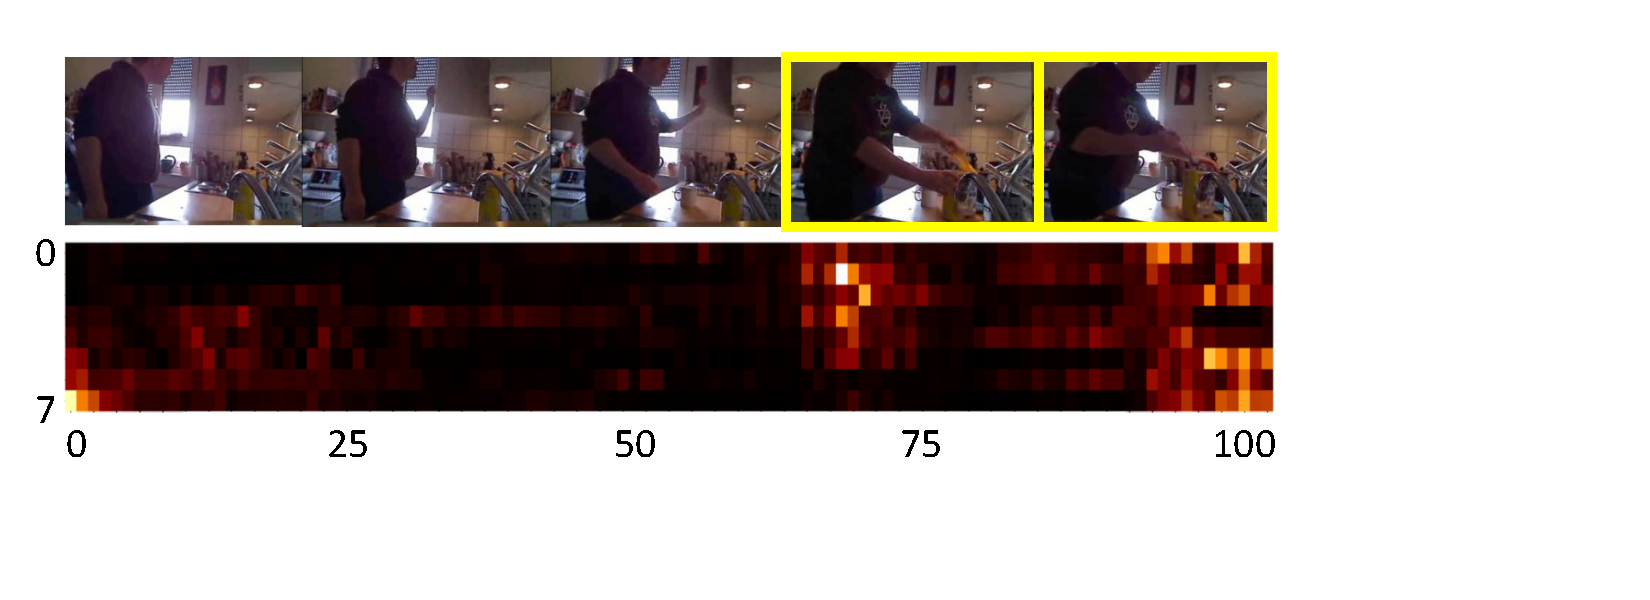
\includegraphics[width=\columnwidth]{Figures/pdf/attn_vis_milk2.pdf}
    \caption{Activity: Milk}
    \label{fig:4b}
    \end{subfigure}
\caption{\textbf{Cross-attention map visualization on Breakfast}. The horizontal and vertical axis indicates the index of the past frames and the action queries, respectively. The brighter color implies a higher attention score. We highlight a video frame with a yellow box where the attention score of the frame is highly activated. RGB frames are uniformly sampled from a video in this figure.}
 \label{fig:4}
\end{figure}